\documentclass{../source/zjureport}

\major{信息工程}
 \name{箫宇 }
\title{实验设计报告}
\stuid{ }
\college{信息与电子工程学院}
\date{\today}
\lab{教7-108}
\course{计算机组成与设计}
\instructor{刘鹏}
\grades{}
\expname{RISC-V指令集仿真器}
\exptype{代码编写}
\partner{无}

\begin{document}
    \makecover
    \makeheader

    \section{代码实现思路}
        \subsection{instforms.cpp}
            我们在informs.cpp文件中的主要工作为实现要求指令的编码函数,即依据函数传入的参数(即寄存器的编号或者立即数),为对应指令类型的结构体进行赋值。

            在赋值的过程中,以encodeLb函数为例讲解代码思路:
            \begin{lstlisting}[language = C , caption = decodeLb]
bool
IFormInst::encodeLb(unsigned rdv, unsigned rs1v, int offset)
{
  //check the reg number
  if(rdv > 31 or rs1v > 31)
    return false;

  if(offset > (1<<11) or -offset < -(1<<11))
    return false;

  fields.opcode = 0x03;
  fields.rd = rdv & 0x1f;
  fields.funct3 = 0x0;
  fields.rs1 = rs1v & 0x1f;

  #pragma GCC diagnostic push
  #pragma GCC diagnostic ignored "-Wconversion"
    fields.imm = offset;
  #pragma GCC diagnostic pop

  return true;
              
            \end{lstlisting}

            可以看到,在函数起始处,需要先对传入的寄存器操作数范围进行检查,因为RISC-V中寄存器数目为32,所以寄存器操作数的值不能超过31。在完成了对寄存器操作数范围的检查后,我们需要检查传入的偏移量offset的范围。

            通过查看union IFormInst的定义可以发现其中定义了结构体fields,然后查阅lb指令的指令结构对fields中的各个成员进行赋值,此处的取与操作是为了再次防止操作数越界。

            代码最后以\#pragma开始的三行代码也是为了再次确保立即数未超出范围。

            \subsection{decode.cpp}
            decode.cpp文件主要关注从1368行开始的decode函数,输入一条指令inst,需要给出其对于的操作数op和指令条目InstEntry。而需要我们完成的部分为l5,l8,l13,l24,l25,l27和l12的部分内容,下面将以l5部分为例讲解代码思路
\begin{lstlisting}[language = C , caption = l5部分]
l5:  // 00101   U-form
    {
        UFormInst uform(inst);
        op0 = uform.bits.rd;
        op1 = uform.immed();
        return instTable_.getEntry(InstId::auipc);
    }
    return instTable_.getEntry(InstId::illegal);
\end{lstlisting}

    通过查阅instforms.hpp中对不同命令的映射,得到op0,op1对应的传入值,将其赋值;如果有funct3,还需要根据funct3值的不同给出不同的InstEntry。如果最终funt3没有与所有指令匹配,则返回illegal。

    \subsection{Hart.cpp}
    Hart.cpp文件主要是功能是实现指令的执行过程,下面将以execAnd为例分析此部分代码的实现思路。
    \begin{lstlisting}[language = c , caption = ]
  template <typename URV>
  void
  Hart<URV>::execAnd(const DecodedInst* di)
  {
    URV v = intRegs_.read(di->op1()) & intRegs_.read(di->op2());
    intRegs_.write(di->op0() , v);
      
  }
    \end{lstlisting}
    
    在这部分代码里面,变量的类型主要分为两种,有符号数$SRV$以及无符号数$URV$。

    主要需要调用的函数有:
    \begin{enumerate}
      \item intRegs_.read():读取寄存器的值
      \item intRegs_.write():在寄存器中写入值
      \item 处理立即数的op0As(URV/SRV)
    \end{enumerate}

    我们需要利用上述函数在Hart.cpp中实现各条指令的执行方式。例如and:将两个源寄存器中的值取出取与在写入目标寄存器中。

\section{调试过程}
    \subsection{单步运行输出信息意义}
    如下图所示,利用交互模式进行单步调试时输出的信息含义如下:
    \begin{figure}[H]
      \centering
      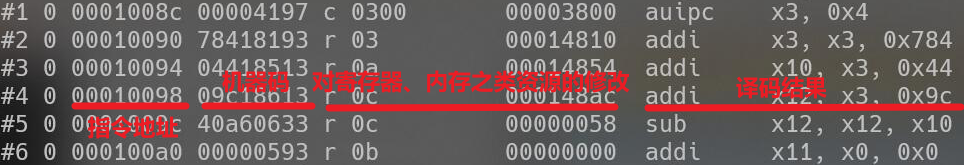
\includegraphics[width = 0.9\textwidth]{figure/debug.png}
      \caption{输出信息}
    \end{figure}
    
    \subsection{调试思路}
    \begin{enumerate}
      \item 可以手动对机器码进行译码操作,看是否和后面的译码结果一样;如果不一致,多半是decode.cpp里面对应的指令有问题
      \item 观察指令对各类资源的修改是否正确;如果不对,有可能是Hart.cpp对应指令有问题
      \item PC指针相关的就看指令地址是否正确跳转
    \end{enumerate}

    \subsection{调试结果}
    \begin{figure}[H]
      \centering
      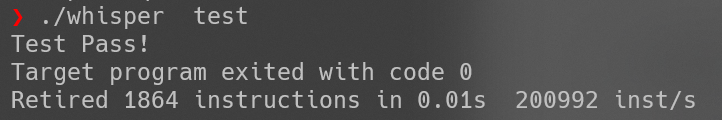
\includegraphics[width = 0.9 \textwidth]{figure/结果.png}
      \caption{测试结果}
    \end{figure}
            
    \section{收获}
    在本次实验中,通过实现部分指令的编码、执行过程,极大地加深了自己对于各种指令的熟悉程度:不仅更加深入地掌握了它的功能,同时也对指令编码有了更深的了解。

    不过对于本次实验也有一些小建议:Project可以搭配Docker镜像一起发布。因为在实验过程中,大部分同学都遇到了诸如boost库无法安装好之类的环境配置问题,花费了大量的时间在编译环境的搭建上。而且最后大家遇到的问题也是千奇百怪,而Docker镜像则是一个很好的解决方案,实测利用镜像可在半小时内搭好环境。可以让大家从环境搭建中解放出来,将精力投入到编码过程中。

\end{document}